\section{Introduction}
The original documentation of the steer-by-wire (sbw) bicycle is incomplete.
This document is an attempt to make the documentation more complete by filling it up with my findings regarding the sbw bicycle.
I also documented the things I added to the sbw bicycle.

Luckily there was already some documentation on this bicycle done by \href{https://github.com/mechmotum/TUDelft-SbW-Bicycle/tree/master/docs}{Simonas Draukas}.
Other documentation on the sbw bicycle can be found in the paper by Georgios Dialynas "Design and implementation of a steer-by-wire bicycle" (2018),
his \href{https://github.com/gdialynas/Steer-by-wire-bicycle}{github repository}, and the master thesis of Christos Christoforidis "Rider control identification in cycling taking into account steer torque feedback and sensorial delays" (2019). 

This document is an extension of the other documentation, so read through them as well.
If there is a contradiction then follow this document, it is the most up-to-date one.

\subsection{Current State of the Bicycle}
Currently the bicycle runs the PD controller as described in Georgios Dialynas's paper.
This controller minimizes the error between the fork and handlebar angle, thereby trying to mimic a mechanical connection.

\subsection{Small Overview}
\begin{figure}[h!]
    \centering
    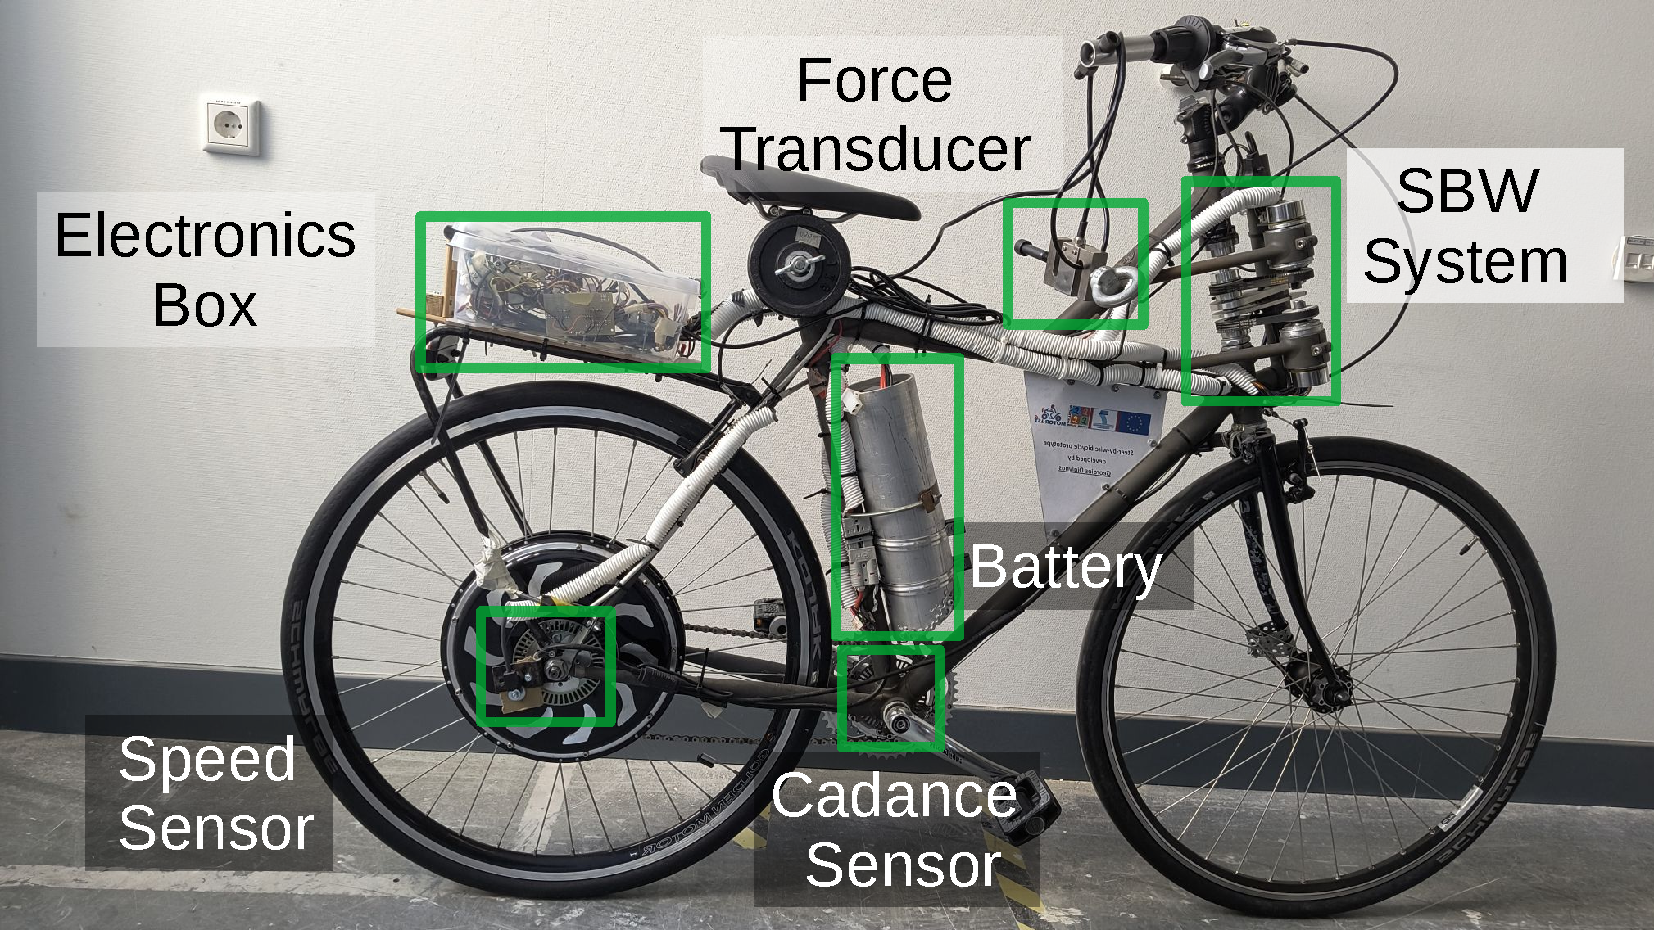
\includegraphics[width=0.99\textwidth]{Img/Overview_of_bicycle.pdf}
    \caption{Overview of the steer-by-wire bicycle}
    \label{fig:sbw_overview}
\end{figure}